\graphicspath{ {./root/1.Inspection/res/} }
\subsection{Final scores}

The following table provides a schematisation of the final scores agreed by all evaluators after discussing each heuristic individually on the \href{https://www.unicef.org/}{UNICEF's website}.
Right below the table, there is a collection of examples, comments and observations that were gathered during the discussion and that aims to justify why the grades have been assigned in this way.

\begingroup
\small
\setlength{\tabcolsep}{1.5cm}
\renewcommand{\arraystretch}{1.35}

\rowcolors{2}{lightgray}{lightblue}
\begin{longtable}{l r}
	
	\hiderowcolors
	\textbf{Heuristic} & \textbf{Score} \\ \hline  \endhead \\
	\showrowcolors
	

	
	\hyperref[subsec:H1]{H1. Visibility of system status} & 2  \\
	\hyperref[subsec:H2]{H2. Match between system and the real world} & 4  \\
	\hyperref[subsec:H3]{H3. User control and freedom} & 3 \\
	\hyperref[subsec:H4]{H4. Consistency and standards} & 2 \\
	\hyperref[subsec:H5]{H5. Error prevention} & 3 \\
	\hyperref[subsec:H6]{H6. Recognition rather than recall} & 4 \\
	\hyperref[subsec:H7]{H7. Flexibility and efficiency of use} & 3 \\
	\hyperref[subsec:H8]{H8. Aesthetic and minimalist design} & 1 \\
	\hyperref[subsec:H9]{H9. Help users recognize, diagnose and recover from errors} & 5 \\
	\hyperref[subsec:H10]{H10. Help and documentation} & 3 \\
	\hyperref[subsec:H11]{H11. Information overload} & 2 \\
	\hyperref[subsec:H12]{H12. Consistency of page content structure}  & 2 \\
	\hyperref[subsec:H13]{H13. Contextualized information} & 2 \\
	\hyperref[subsec:H14]{H14. Content organisation (hierarchy)} & 4 \\
	\hyperref[subsec:H15]{H15. Interaction consistency} & 1 \\
	\hyperref[subsec:H16]{H16. Group navigation-1} & 2 \\
	\hyperref[subsec:H17]{H17. Group navigation-2} & 3 \\
	\hyperref[subsec:H18]{H18. Structural navigation} & 3 \\
	\hyperref[subsec:H19]{H19. Semantic navigation} & 4 \\
	\hyperref[subsec:H20]{H20. “Landmarks”} & 3 \\
	\hyperref[subsec:H21]{H21. Text lay out} & 4 \\
	\hyperref[subsec:H22]{H22. Interaction placeholders-semiotics} & 3 \\
	\hyperref[subsec:H23]{H23. Interaction placeholders-consistency} & 1 \\
	\hyperref[subsec:H24]{H24. Consistency of visual elements} & 3 \\
	\hyperref[subsec:H25]{H25. Hierarchy-1} & 3 \\
	\hyperref[subsec:H26]{H26. Hierarchy-2} & 2 \\
	\hyperref[subsec:H27]{H27. Spatial allocation-1} & 4 \\
	\hyperref[subsec:H28]{H28. Spatial allocation-2} & 4 \\
	\hyperref[subsec:H29]{H29. Consistency of page spatial structure} & 3 \\
	
	
	
\end{longtable}

\endgroup


\clearpage



\section*{Comments on the scores}
\paragraph{H1. Visibility of system status - Score 2} \label{subsec:H1}	
The reasons for the low grade associated to this heuristic are several. Firstly, breadcrumbs are provided only in a very little subset of pages, to assist users in understanding their current location, but they are missing most of the times. Here is a picture representing the way breadcrumbs are shown on UNICEF's website:
\begin{figure}[!h]
	\begin{center}
		
\includegraphics[width=0.5\textwidth]{FinalScores1.jpg}
		\captionsetup{font=small}
		\caption{\textit{Example of breadcrumb.}}
	\end{center}
\end{figure}
\newline Another relevant issue is that the section of the navigation bar on top of the page in which the user is located is not highlighted in any way, making it difficult for users to recognize what part of the website they're exploring.
\begin{figure}[!h]
	\begin{center}
		
\includegraphics[width=0.6\textwidth]{FinalScores2.jpg}
		\captionsetup{font=small}
		\caption{\textit{The navigation bar does not highlight.}}
	\end{center}
\end{figure}
\newline
Moreover, disorientation is also caused by the different behaviours of links inside the website. For instance, when looking at the navigation bar, there are some links that lead the user to a new page still contained inside \href{https://www.unicef.org/}{UNICEF global}, while others redirect the user to a sub-page that is distinct from the global one and in which the fundamental landmarks and reference points change. Here's an example that can be tested by clicking on the link \href{https://www.unicef.org/innovation/}{"Innovation"} inside the navigation bar.
\begin{figure}[!h]
	\begin{center}
		
\includegraphics[width=0.7\textwidth]{FinalScores3.jpg}
		\captionsetup{font=small}
		\caption{\textit{Example of different website similar to the original one.}}
	\end{center}
\end{figure}
The new page presents completely different buttons, a new navigation bar with different sections from the one in the global website, and also the landmark for going back to the home page changes behaviour (it leads to this new home page instead of \href{https://www.unicef.org/}{UNICEF global}).







%------------------------------H2------------------------------------






\paragraph{H2. Match between system and the real world - Score 4} \label{subsec:H2}	In general, the language used on the website matches the user’s existing knowledge and mental models, making it easy for him/her to understand the information provided. Also, the icons used on the website represent familiar concepts, facilitating the comprehension.
\begin{figure}[!h]
	\begin{center}
		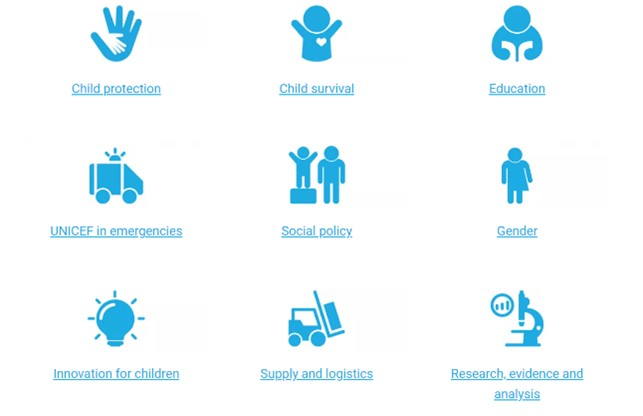
\includegraphics[width=0.4\textwidth]{FinalScores4.jpg}
		\captionsetup{font=small}
		\caption{\textit{Example of familiar icons and language.}}
	\end{center}
\end{figure}
\newline However, there are instances where the adopted solutions are not so clear and straightforward, as it can be observed in the page \href{https://www.unicef.org/where-we-work}{Where we work}. For example, the “Browse areas by alphabetical listing” section could have been designed in a more intuitive way for the users to understand that it was a classifications of countries by alphabetical order.
\begin{figure}[!h]
	\begin{center}
		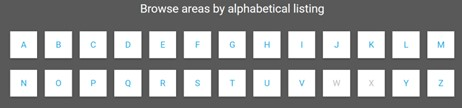
\includegraphics[width=0.7\textwidth]{FinalScores5.jpg}
		\captionsetup{font=small}
		\caption{\textit{Bad and unfamiliar listing of areas.}}
	\end{center}
\end{figure}
\newline
\newline
It has to be mentioned also the fact that there is a not-functioning button labelled “Join UNICEF” on the page for  \href{https://www.unicef.org/partnerships}{Partnerships}. The problem related to this heuristic here is the fact that the communication of the error is quite technical and not suitable with a user without any experience in computer science of IT technologies.












%----------------------------H3--------------------------------------








\paragraph{H3. User control and freedom - Score 3} \label{subsec:H3}	The grade is at the centre of the scale as there are positive and negative aspects to be discussed for this heuristic. Good examples of user control implemented on the website are the search engines spread across the website. Indeed, users can engage with these search engines by applying filters, removing them and so on. In \hyperref[fig:job]{Figure 6}, a picture of the search engine for job opportunities is provided, but also the other ones on the website have similar capabilities. 
\begin{figure}[!h]
	\label{fig:job}
	\begin{center}
		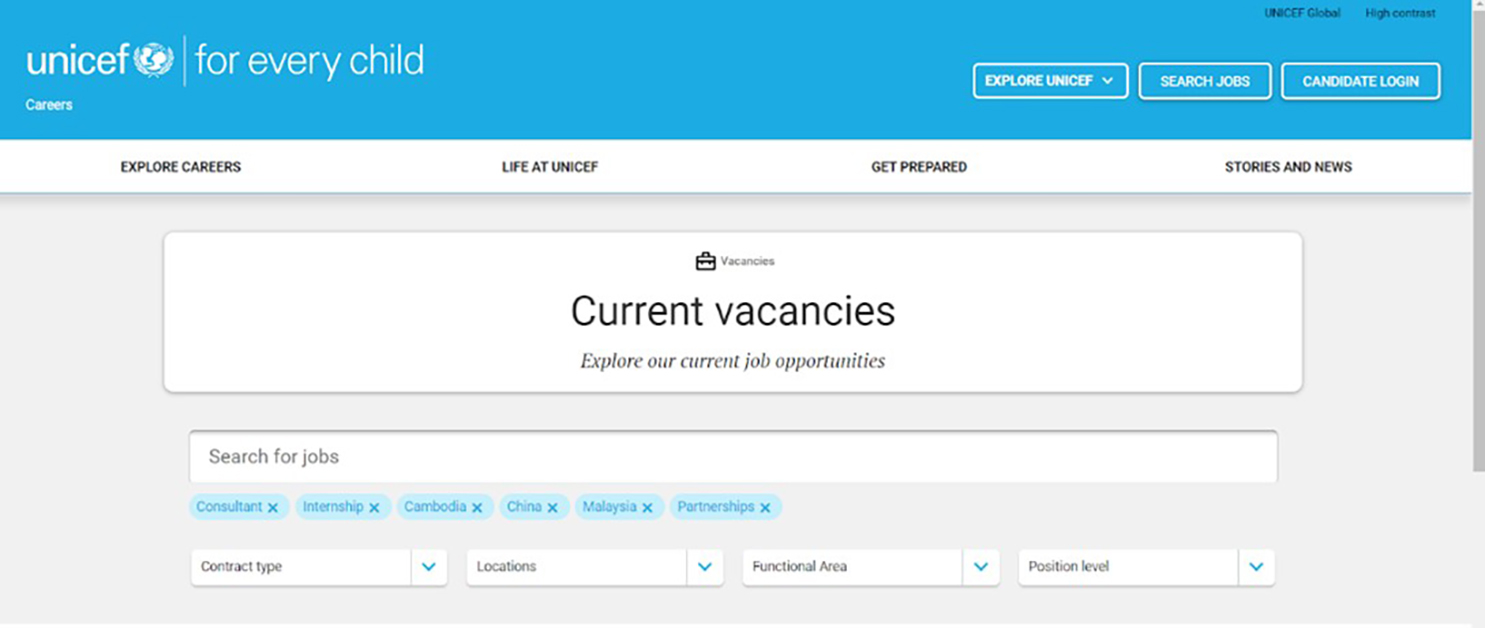
\includegraphics[width=0.7\textwidth]{FinalScores6.jpg}
		\captionsetup{font=small}
		\caption{\textit{Search engine for job opportunities.}}
	\end{center}
\end{figure}
\newline On the other hand, in some sections of the website user's freedom is limited.
As already mentioned for the heuristic \hyperref[subsec:H1]{H1. Visibility of system status}, some sub-pages of the website trap the user in and make it difficult to go back to the \href{https://www.unicef.org/}{UNICEF global} page.

Furthermore, during the donation process, the ‘undo’ feature is implemented but it requires the user to insert all data again every time.

Also, when trying to change page from the donation page, a big message appears on the screen to catch the user's attention and prevent them from going away. While this feature might have been purposely implemented, it undermines the user's sense of freedom.
\begin{figure}[!h]
	\begin{center}
		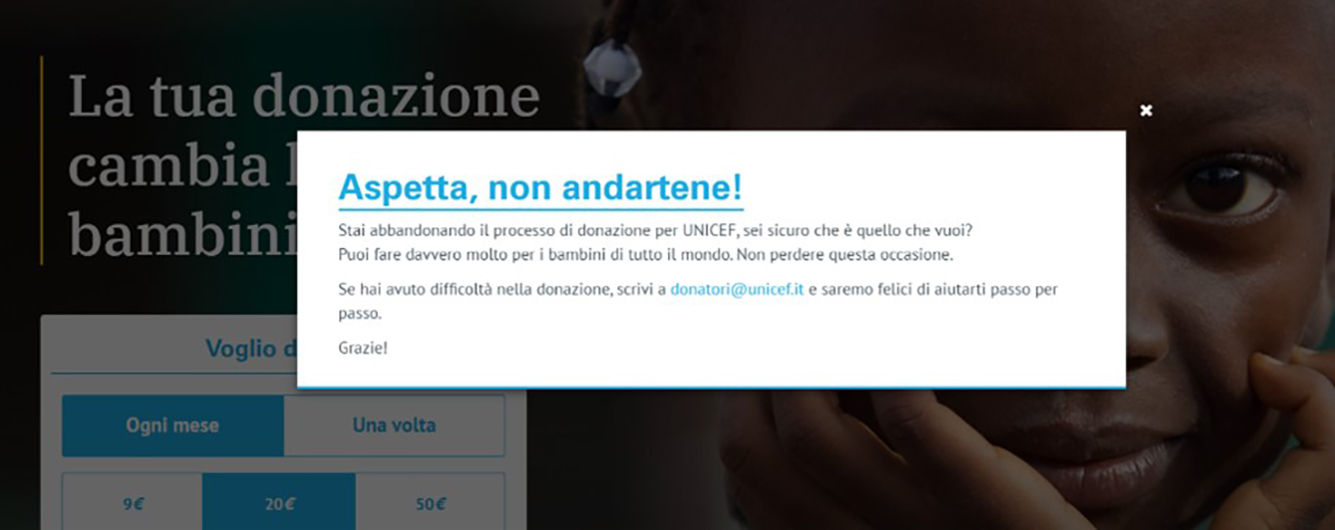
\includegraphics[width=0.7\textwidth]{FinalScores7.jpg}
		\captionsetup{font=small}
		\caption{\textit{A big message appears on the screen.}}
	\end{center}
\end{figure}





%----------------------------H4--------------------------------------


\paragraph{H4. Consistency and standards - Score 2} \label{subsec:H4}	The reason for the low grade is the fact that from a high-level point of view there is consistency between similar pages and some standards are respected, but there are also many problems to be pointed out.
\newline The "donate" button is highly inconsistent across the entire website (it takes different shapes and labels depending on the page), and it is red-coloured, which might not be the best standard for the purpose of the button, as it might lead to a sense of angriness or alarm for the user.
\begin{figure}[!h]
	\begin{center}
		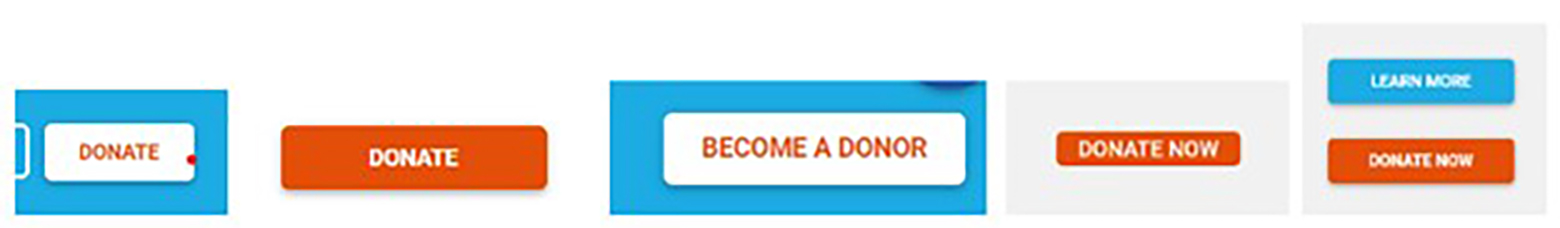
\includegraphics[width=0.7\textwidth]{FinalScores8.jpg}
		\captionsetup{font=small}
		\caption{\textit{Examples of donate buttons.}}
	\end{center}
\end{figure}
\newline Besides, the cards that are used to present articles or publications sometimes present different icons or colours. This can be seen in \hyperref[fig:cards]{Figure 9}
\begin{figure}[!h]
	\label{fig:cards}
	\begin{center}
		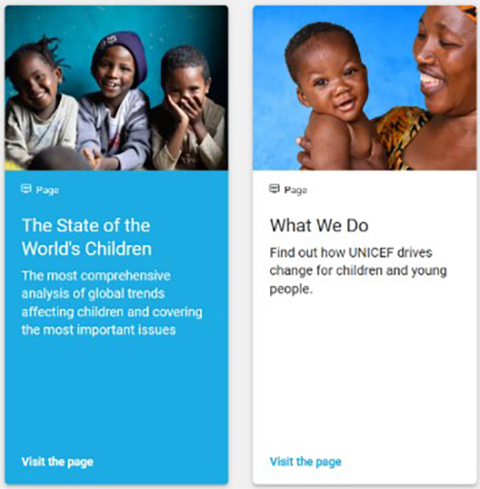
\includegraphics[width=0.4\textwidth]{FinalScores9.jpg}
		\captionsetup{font=small}
		\caption{\textit{Inconsistency between cards.}}
	\end{center}
\end{figure}

In some cases, similar icons are used to express different concepts. In \hyperref[fig:fig10]{Figure 10}, two light bulb icons are displayed and they're used to convey different concepts in two separated pages of the website.


\begin{figure}[!h]
	\label{fig:fig10}
	\begin{center}
		
\includegraphics[width=0.4\textwidth]{FinalScores10.jpg}
		\captionsetup{font=small}
		\caption{\textit{Similar icons for different meanings.}}
	\end{center}
\end{figure}
It is also possible to notice inconsistencies in the way the donation option is provided to the user. When clicking on a DONATE button from the \href{https://www.unicef.org/}{UNICEF global} webpage, the user is redirected to a donation page where it is possible to support UNICEF as an agency (general donation). Conversely, by looking at the sub-pages under "Stories" section in the navigation bar, it is possible to spot some cases in which the donation is handled differently. For instance, on the page for the \href{https://www.unicef.org/emergencies/delivering-support-afghanistans-children}{Afghanistan's emergency}, the donation button leads to a specific donation for supporting the Afghanistan's crisis, which is different from the one on the global page.
\newline 
Finally, by inspecting the website closely, some non-standard and unintuitive icons can be noticed. For example, on the page dedicated to  \href{https://www.unicef.org/algeria/agir}{Algeria}, there is a very unconventional icon representing a sort of laptop whose meaning is very difficult to grasp. It redirects the user to the homepage of the website for Algeria.
\begin{figure}[!h]
	\begin{center}
		
\includegraphics[width=0.5\textwidth]{FinalScores11.jpg}
		\captionsetup{font=small}
		\caption{\textit{Very strange and unfamiliar icon (the last one on the right).}}
	\end{center}
\end{figure}




%----------------------------H5------------------------------------




\paragraph{H5. Error prevention - Score 3}  \label{subsec:H5}	In the donation page, when filling out the form, there is no double check for the user's email or a pop up to encourage the user to check again their data for both personal and bank/card.
In this page it is neither showed the minimum quote of donation, which means a missing error prevention.
\newline In the contact page of the section ‘UNICEF data’ (\href {https://data.unicef.org/contact/}{https://data.unicef.org/contact/}) there is a series of fields to fill in, if some of them are incorrectly filled no error message appears, when you click submit all errors appear.
\newline In general, this website is mainly for consulting information and does not offer many interactions with the users that could lead to error-prone situations.
\newline
\newline \paragraph{H6. Recognition rather than recall - Score 4}  \label{subsec:H6}	Recognition is present when the user uses the search bar.
\begin{figure}[!h]
	\begin{center}
		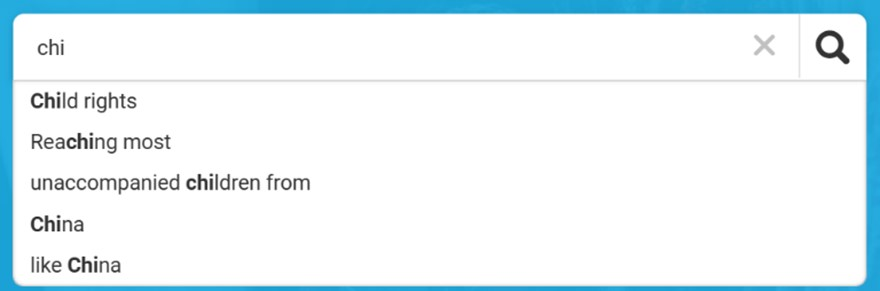
\includegraphics[width=0.5\textwidth]{FinalScores12.jpg}
		\captionsetup{font=small}
		\caption{\textit{Recognition provided in the search bar.}}
	\end{center}
\end{figure}
\newline The drop-down menus also help to recognize by offering a list of options for the main topics. 
\newline In general, all needed information for a specific topic is provided in a single page.
\newline Despite these positive aspects, there are some pages too nested and too difficult to find even with the search bar (e.g. The Skills4Girls page).
\newline
\newline \paragraph{H7. Flexibility and efficiency of use - Score 3} \label{subsec:H7}	The website's efficiency is not too bad, in fact the most relevant landmarks are on the page, the problem is that there are only these few web accelerators, which are also less visible.
\begin{figure}[!h]
	\begin{center}
		
\includegraphics[width=0.4\textwidth]{FinalScores13.jpg}
		\captionsetup{font=small}
		\caption{\textit{Examples of less visible landmarks.}}
	\end{center}
\end{figure}
\newline In terms of flexibility, no customization or personalization is possible across the website, and the interface is difficult to learn, very complex and full of information, making it hard for less experienced users to easily find the information needed. It is neither good for an experienced user, which would like to have a personal section where save articles or frequently visited pages.
\newline
\newline \paragraph{H8. Aesthetic and minimalist design - Score 1} \label{subsec:H8}	The interface is not simple or functional, as it is cluttered with many different design elements that often deviate from an established design system. In this way the interface is not supporting the users’ primary goals due to the overload of information.
\newline UNICEF website is complex, due to the need of presenting many different information that support and explain the cause, but its visual design is not focused on the essential and this tragically compromises the user experience.
\newline Some examples are the page \href{https://www.unicef.org/reports/state-worlds-children-2023}{https://www.unicef.org/reports/state-worlds-children-2023} and the not essential quiz in the page \href{https://www.unicef.org/on-my-mind}{OnMyMind: Better mental health for every child | UNICEF} which could have been hidden instead of filling the whole screen. 
\begin{figure}[!h]
	\begin{center}
		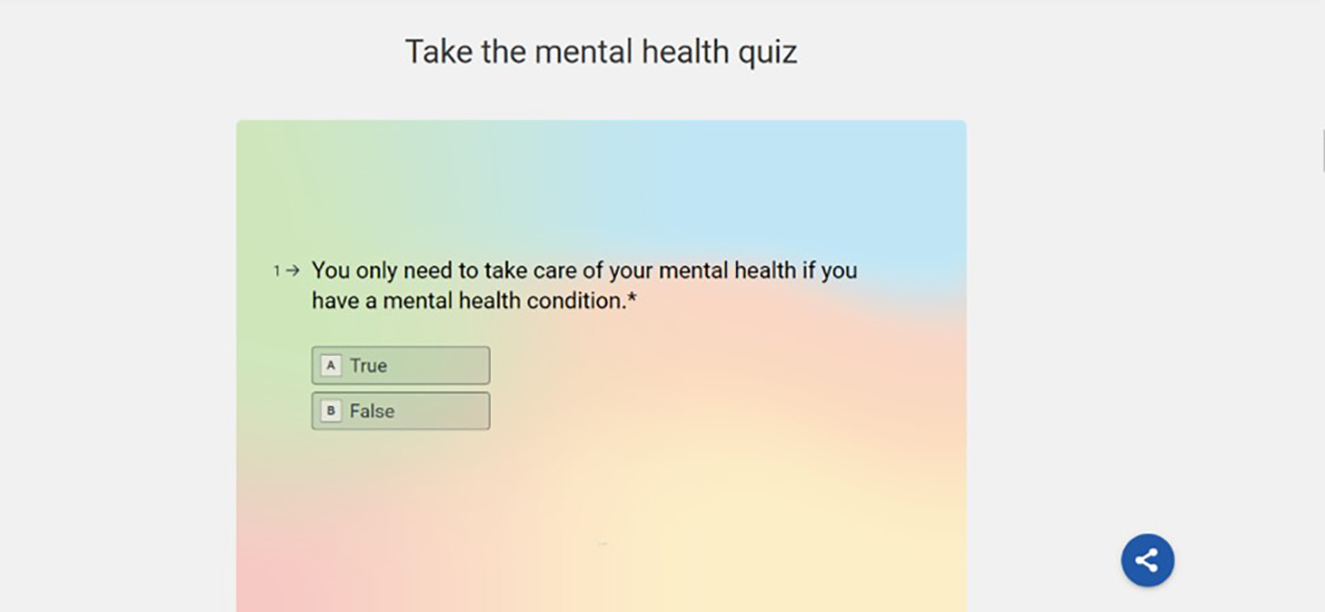
\includegraphics[width=0.6\textwidth]{FinalScores14.jpg}
		\captionsetup{font=small}
		\caption{\textit{Big and unaesthetic quiz.}}
	\end{center}
\end{figure}
\newline
\newline \paragraph{H9. Help users recognize, diagnose and recover from errors - Score 5} \label{subsec:H9}	Mistakes when filling forms are correctly highlighted, they are expressed in plain language (no error codes), precisely indicating the problem, and constructively suggesting a solution.
\begin{figure}[!h]
	\begin{center}
		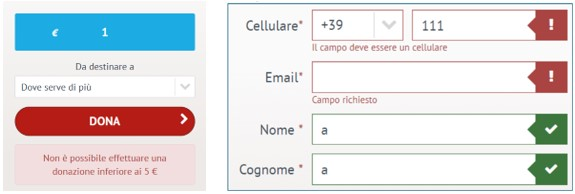
\includegraphics[width=0.7\textwidth]{FinalScores15.jpg}
		\captionsetup{font=small}
		\caption{\textit{Errors recognizing.}}
	\end{center}
\end{figure}
\newline
\newline \paragraph{H10. Help and documentation - Score 3}  \label{subsec:H10}	Help and documentation are well provided by the FAQ page and the contact us page, but they are too difficult to find.
\newline
\newline \paragraph{H11. Information overload - Score 2}  \label{subsec:H11}	Really often, in the various pages of the website, there are so many unnecessary information, images, links and other elements, this lack of conciseness creates difficulties in achieving the tasks. A clear example is the page \href{https://www.unicef.org/reports/state-worlds-children-2023}{https://www.unicef.org/reports/state-worlds-children-2023}.
\newline In only a few cases, information is correctly divided by colours/sections, and some pages are still acceptable, like the home page \href{https://www.unicef.org/}{UNICEF} or the donation page (\href{https://donazioni.unicef.it}{Una donazione per aiutare i bambini - Comitato Italiano per l'UNICEF Fondazione ETS}).
\newline
\newline \paragraph{H12. Consistency of Page Content Structure - Score 2}  \label{subsec:H12}	In some pages of the same type there is consistency, for example the two pages \href{https://www.unicef.org/gender-equality}{Gender equality | UNICEF} and \href{https://www.unicef.org/health}{Health | UNICEF} have the same style and structure.
\newline However, there are many pages of the same type where the structure is not consistent and contains different types of elements, this happens, for example, in pages of the ‘Focus Area’ section.
\newline Also, in the 'Stories' section, all the pages have a different donation section, creating inconsistency among them.
\begin{figure}[!h]
	\begin{center}
		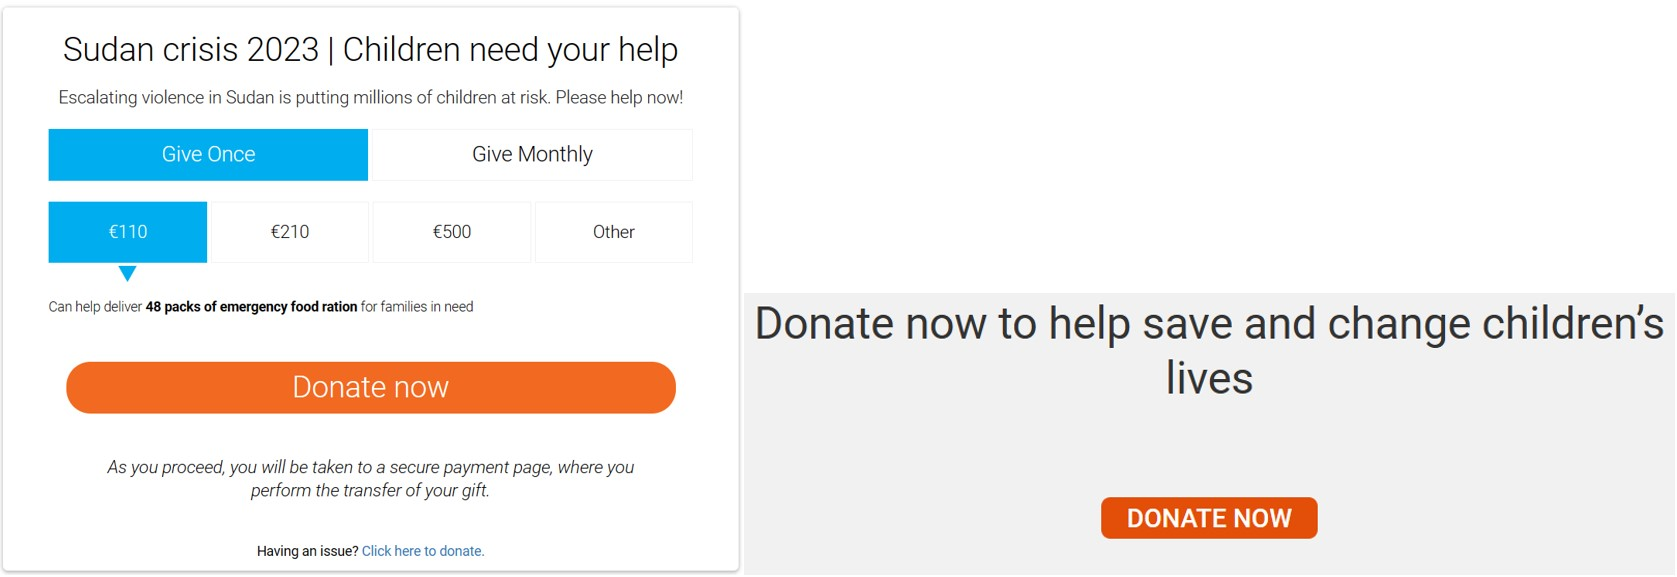
\includegraphics[width=0.9\textwidth]{FinalScores16.jpg}
		\captionsetup{font=small}
		\caption{\textit{Inconsistency between two donate sections.}}
	\end{center}
\end{figure}
\newline
\newline \paragraph{H13. Contextualized Information - Score 2}  \label{subsec:H13}	Some elements can help users to understand where they are, for example the title or the image at the top of each page, but it is not enough.
\begin{figure}[!h]
	\begin{center}
		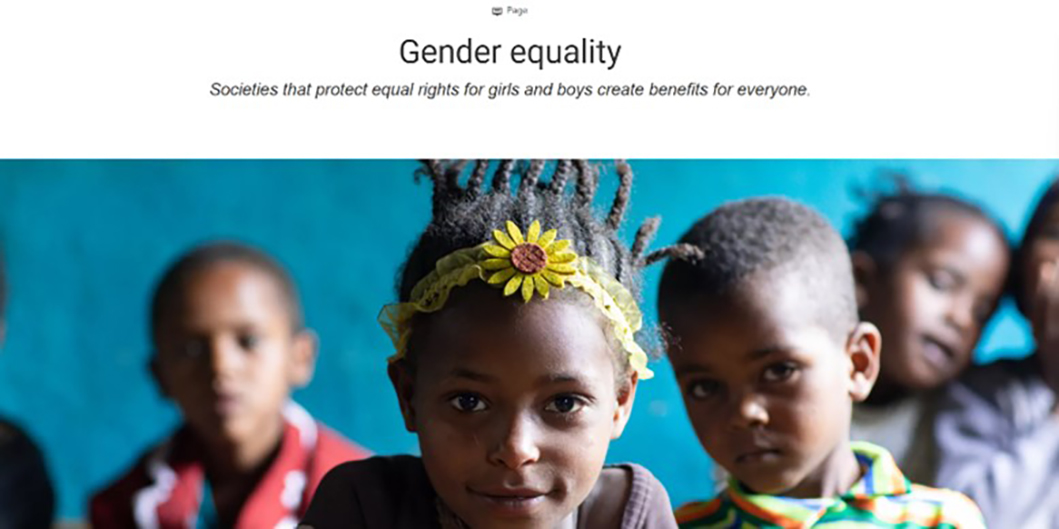
\includegraphics[width=0.7\textwidth]{FinalScores17.jpg}
		\captionsetup{font=small}
		\caption{\textit{Example of title and image of a page.}}
	\end{center}
\end{figure}
\newline Breadcrumbs at the top of the pages are not consistent, they are present only on a few pages, these elements could help users if they were always available.
\newline Also, highlighting the name of the menu in which the user is located would provide further assistance.
\newline
\newline \paragraph{H14. Content organization (hierarchy) - Score 4}  \label{subsec:H14}	The content is organized in an understandable manner, even it is not the most intuitive and it can generate a bit of confusion.
\newline The hierarchy is mainly represented by the main 5 section of the menu, the subsections of each of them, and then there are hierarchical relations inside some pages.   
\begin{figure}[!h]
	\begin{center}
		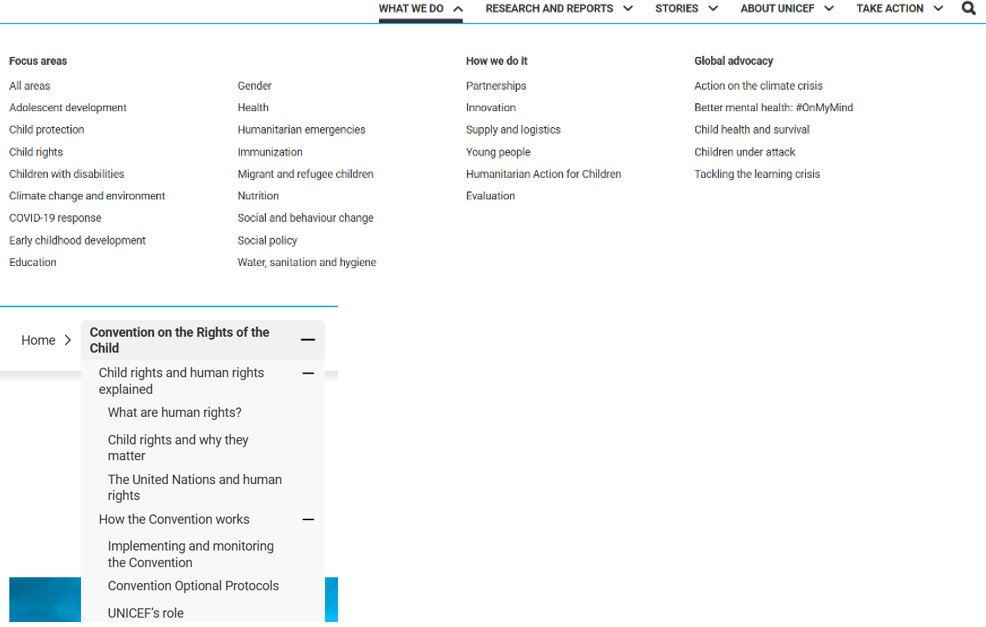
\includegraphics[width=\textwidth]{FinalScores18.jpg}
		\captionsetup{font=small}
		\caption{\textit{Elements which provide hierarchy in the website.}}
	\end{center}
\end{figure}
\newline
So, sections and categories are well organized, but sometimes they are redundant in the hierarchy since they may belong to various sections, like \href{https://www.unicef.org/partnerships}{UNICEF partnerships | UNICEF} which belongs both to “Take action” and “What we do”, even though it could have been present in only the first instance. 
\newline A negative aspect is the frequent occurrence of links on pages that don't fit into a precise hierarchy but are only accessible in this manner.
\newline
\newline \paragraph{H15. Interaction consistency - Score 1}	\label{subsec:H15}The menu should be always the same, but there are pages in which it is totally different, in fact the two pages \href{https://www.unicef.org/careers/}{UNICEF Careers | UNICEF Careers} and \href{https://www.unicef.org/partnerships}{UNICEF partnerships | UNICEF} have different menus. Even changing the language leads to pages with different menus and different interactions with them (they are no more drop-down menus).
\newline Additionally, between pages of the same type, there are different ways to interact, for example, some pages include 'Our Focus Areas' while others do not, and some have a navigable index while others do not.
\begin{figure}[!h]
	\begin{center}
		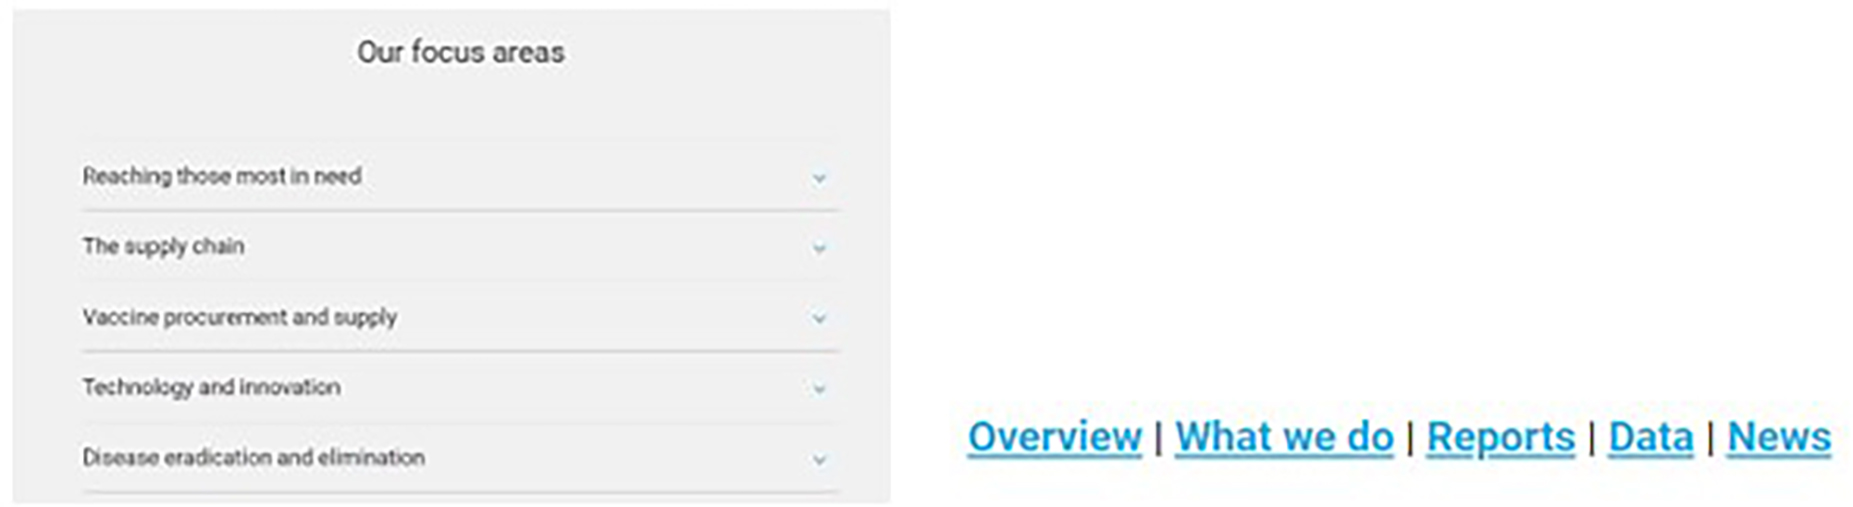
\includegraphics[width=0.8\textwidth]{FinalScores19.jpg}
		\captionsetup{font=small}
		\caption{\textit{The "Our focus areas" element and the navigable index.}}
	\end{center}
\end{figure}
\newline And again, the interaction with the donation section on each page is different.
\newline
\newline \paragraph{H16. Group navigation-1 - Score 2}  \label{subsec:H16}	When breadcrumbs are present, navigating within a specific topic is relatively easy. However, on most of the website, breadcrumbs are absent, and as a result, it is easy to navigate from general sections to subpages, but not the other way around, nor among subpages. For example, when visiting a related article from a page, it is difficult to go back.
\newline We also noticed that articles cannot be viewed in chronological order, and there is generally no clear order between articles. Consequently, there is no option, for example, to move to the next article.
\newline Overall, the navigation experience is confusing.
\newline
\newline \paragraph{H17. Group navigation-2 - Score 3}  \label{subsec:H17}	The main menu contains a lot of information, but it is generally intuitive and clear, with sections clearly differentiated by consistent names that match the real world and an appropriate font size. However, there are some inconsistencies like the titles of the menus which are links to some pages, or names presented differently when opening the page. These discrepancies may create cognitive load. 
\newline In addition, there are some links that lead to different websites and it’s not clear until the user clicks on them, this also create confusion.
\begin{figure}[!h]
	\begin{center}
		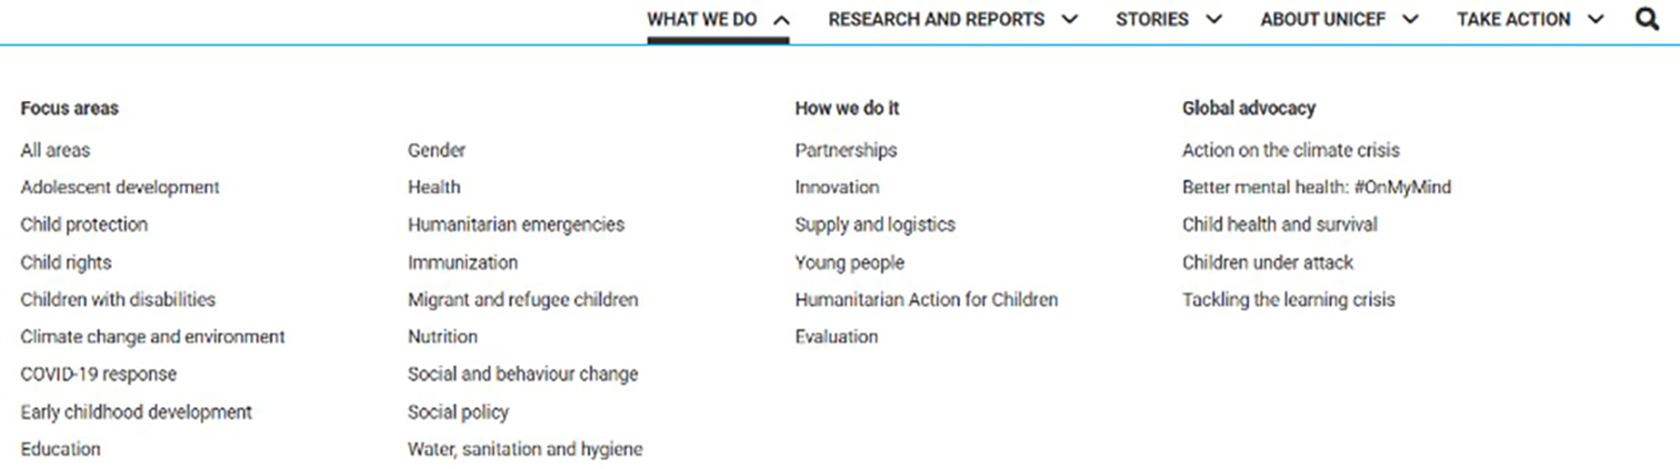
\includegraphics[width=\textwidth]{FinalScores20.jpg}
		\captionsetup{font=small}
		\caption{\textit{The main menu of the website.}}
	\end{center}
\end{figure}
\newline
\newline \paragraph{H18. Structural Navigation - Score 3}  \label{subsec:H18}	It’s easy enough to navigate among components of a single topic (a single page), but usually, the navigation between a topic and his related articles is quite complex, in fact after opening a link, usually it’s not possible to go back.
\newline A negative aspect of the navigation in a single topic is the lack of hierarchy, which does not help users to understand which part to prioritize: usually similar size and same font for all the elements of a single page.
\newline An example of bad navigation in a page is \href{https://www.unicef.org/reports/state-worlds-children-2023}{https://www.unicef.org/reports/state-worlds-children-2023}, where even background images create confusion.
\newline
\newline \paragraph{H19. Semantic Navigation - Score 4}  \label{subsec:H19}	Usually, similar topics are grouped and linked via a new drop-down menu, which makes it easy to navigate among related topics in both directions, but this happens only for some pages.
\begin{figure}[!h]
	\begin{center}
		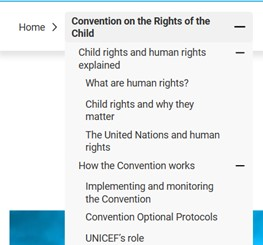
\includegraphics[width=0.3\textwidth]{FinalScores21.jpg}
		\captionsetup{font=small}
		\caption{\textit{Example of drop-down menu which groups similar topics.}}
	\end{center}
\end{figure}
\newline In some pages, there are also sections like ‘related topics’ or ‘find out more’ which help to navigate from a topic to a related one, but not vice-versa.
\begin{figure}[!h]
	\begin{center}
		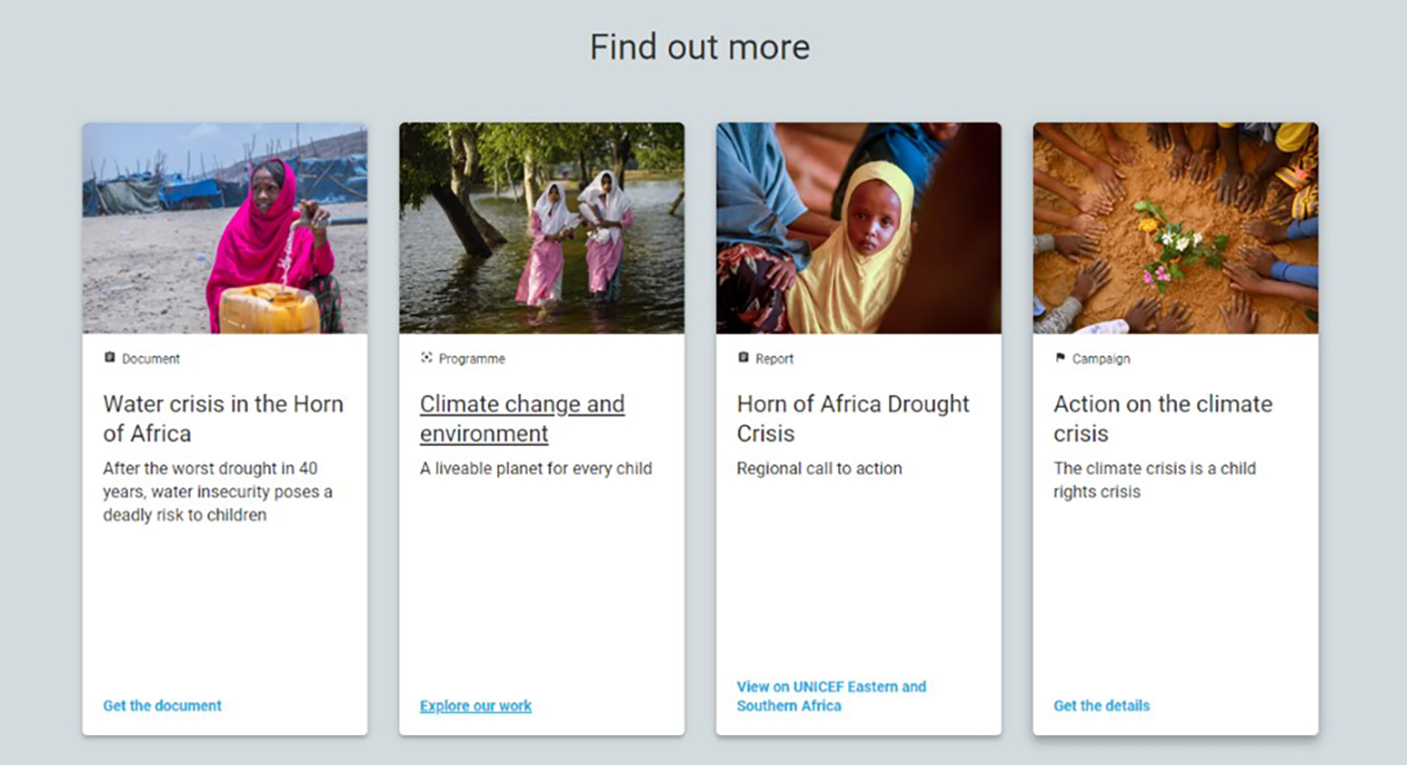
\includegraphics[width=0.7\textwidth]{FinalScores22.jpg}
		\captionsetup{font=small}
		\caption{\textit{Example of 'Find out more' section.}}
	\end{center}
\end{figure}
\newline
\newline \paragraph{H20. “Landmarks” - Score 3}	\label{subsec:H20}In general, landmarks provide a fast access to the main parts of the website, both in the header and in the footer, but most of them are less visible and difficult to find, such as the ‘contact us’ in the footer.
\newline There is also an issue with the home landmark: sometimes happens that the user reaches a different section of the website and the destination of the home landmark change. For example the home landmark of the page \href{https://www.unicef.org/careers/}{UNICEF Careers | UNICEF Careers} does not take to the true home page of the website, but there is a different landmark that is less visible and less intuitive.
\begin{figure}[!h]
	\begin{center}
		
\includegraphics[width=0.6\textwidth]{FinalScores23.jpg}
		\captionsetup{font=small}
		\caption{\textit{Less visible landmark to go back to UNICEF global.}}
	\end{center}
\end{figure}
\newline Some positive features include the presence of a landmark to share an article, which is always present in the bottom-right of the screen, and the menu which scrolls down with the user, unfortunately it’s not the same for the logo.
\newline
\newline \paragraph{H21. Text lay out - Score 4}  \label{subsec:H21}	In general, the font size is appropriate and the text is readable, there are only few elements that are less visible.
\begin{figure}[!h]
	\begin{center}
		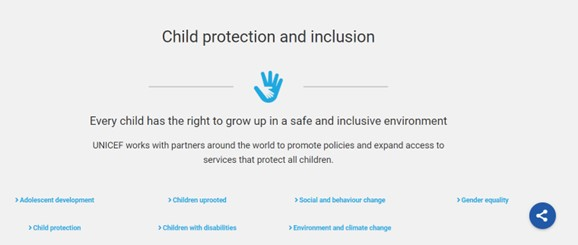
\includegraphics[width=0.8\textwidth]{FinalScores24.jpg}
		\captionsetup{font=small}
		\caption{\textit{Examples of less visible elements.}}
	\end{center}
\end{figure}
\newline In addition, the text of the body could be a little smaller to give a better visual hierarchy in the pages.
\newline
\newline \paragraph{H22. Interaction placeholders-semiotics - Score 3}  \label{subsec:H22}	There are many intuitive elements on the website, such as links which are coloured and underlined when overlaying with the mouse, and clickable cards which have an overlay shadow, as well as textual and primary buttons.
\newline However, there are also some less intuitive elements:
\newline -	The drop-down menus are also links.
\newline -	Many other links are unclear in terms of where they lead or whether they open a new website.
\newline -	The ‘data and insight’ section of some pages contains icons which are clickable links, but they don’t seem links at all.
\begin{figure}[!h]
	\begin{center}
		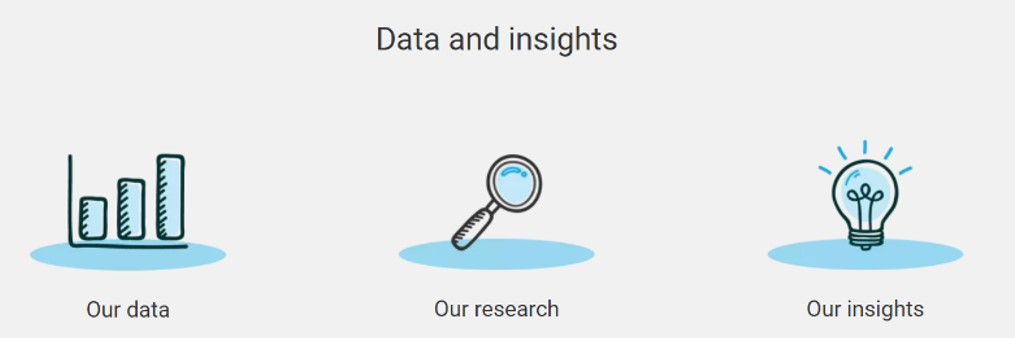
\includegraphics[width=0.5\textwidth]{FinalScores25.jpg}
		\captionsetup{font=small}
		\caption{\textit{The ‘data and insight’ section.}}
	\end{center}
\end{figure}
\newline -	On the page \href{https://www.unicef-irc.org/}{https://www.unicef-irc.org/} there is a functionality to modify the font size which is less intuitive.
\begin{figure}[!h]
	\begin{center}
		
\includegraphics[width=0.4\textwidth]{FinalScores26.jpg}
		\captionsetup{font=small}
		\caption{\textit{Less intuitive functionality to modify the font size.}}
	\end{center}
\end{figure}
\newline
\newline \paragraph{H23. Interaction placeholders-consistency - Score 1}  \label{subsec:H23}	There are many inconsistent visual elements. For example, the 'donate' button and cards often change.
\begin{figure}[!h]
	\begin{center}
		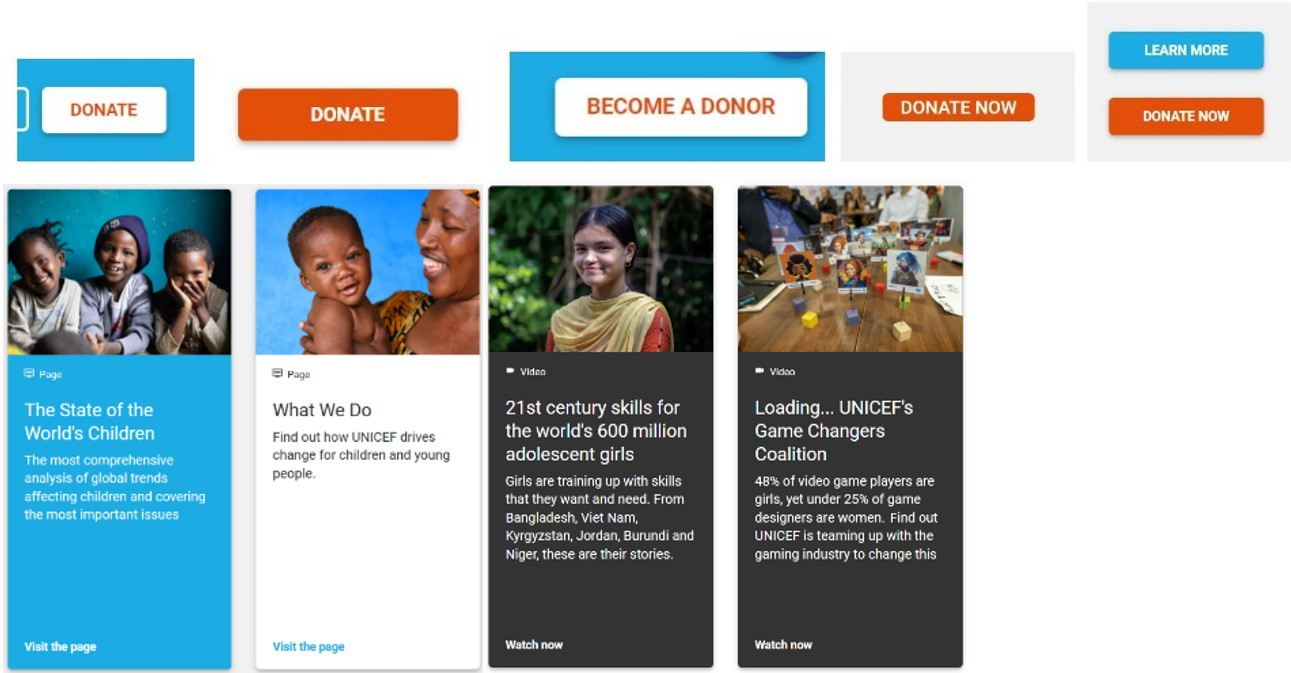
\includegraphics[width=0.8\textwidth]{FinalScores27.jpg}
		\captionsetup{font=small}
		\caption{\textit{Examples of inconsistent visual elements.}}
	\end{center}
\end{figure}
\newline There is inconsistency in how videos are presented in the page, sometimes they are links and sometimes they are integrated in the page.
\newline Also reports presents inconsistency because interactions in reports are totally different from interactions of other pages.
\newline
\newline \paragraph{H24. Consistency of Visual Elements - Score 3}  \label{subsec:H24}	In pages of the same type there is some consistency between visual elements in the sense that they have the same visual properties, but there are also elements which create confusion.
\newline As already mentioned, the inconsistency of the donate buttons and the menus in different pages of the website create confusion in the user, but also cards often have different visual properties: some cards have no images, other are missing of the title or the description.
\begin{figure}[!h]
	\begin{center}
		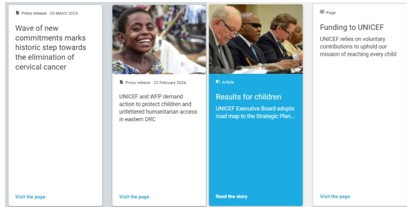
\includegraphics[width=0.7\textwidth]{FinalScores28.jpg}
		\captionsetup{font=small}
		\caption{\textit{Different visual properties between cards.}}
	\end{center}
\end{figure}
\newline The resources associated with different articles also vary in properties. Sometimes they are showed with simple links, other times with tables or more complicated links.
\begin{figure}[!h]
	\begin{center}
		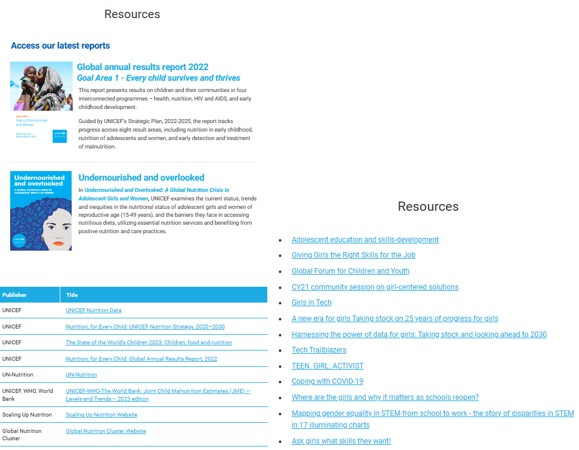
\includegraphics[width=\textwidth]{FinalScores29.jpg}
		\captionsetup{font=small}
		\caption{\textit{Examples of different ways to show resources.}}
	\end{center}
\end{figure}
\newline
\newline \paragraph{H25. Hierarchy-1 - Score 3}  \label{subsec:H25}	The vertical order of elements on the pages contributes to providing a sense of hierarchy. On the contrary, the dimensions of various elements throughout the page are often the same, even the text size is often the same in both important and less relevant elements, this does not help to hierarchy.
\newline
\newline \paragraph{H26. Hierarchy-2 - Score 2}	\label{subsec:H26} Some important elements, such as the logo in the top-left corner and the always-visible donate button at the top of the page, have the appropriate relevance.
\newline However, all visual elements occupy nearly the same amount of space on the page, regardless of their relevance. This lack of hierarchy makes it difficult for users to distinguish between important and less important elements. 
\newline The positioning and sizing of cards throughout the pages create confusion for users in determining which elements are most important.
\newline Also the text in different visual elements is often the same, but the relevance of them should be different.
\newline
\newline \paragraph{H27. Spatial allocation-1 - Score 4} \label{subsec:H27}	Generally, semantically related elements are positioned close to each other.
\begin{figure}[!h]
	\begin{center}
		
\includegraphics[width=0.4\textwidth]{FinalScores30.jpg}
		\captionsetup{font=small}
		\caption{\textit{Examples of related elements.}}
	\end{center}
\end{figure}
\newline Only few elements are bad positioned, one example is the ‘contact us’ landmark which is expected to be located in the drop-down menu ‘about UNICEF’ because they are semantically related, but it is in the footer, so distant.
\newline
\newline \paragraph{H28. Spatial allocation-2 - Score 4} \label{subsec:H28}	Semantically distant elements are typically divided with sections of different colors, often grey, but the body font size makes it hard to distinguish between each section. 
\begin{figure}[!h]
	\begin{center}
		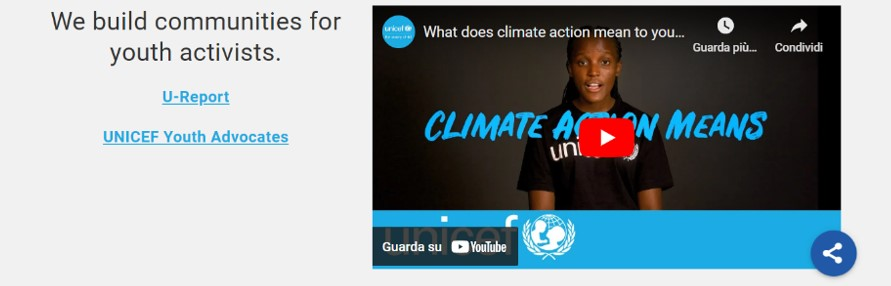
\includegraphics[width=0.6\textwidth]{FinalScores31.jpg}
		\captionsetup{font=small}
		\caption{\textit{Different background colours for different sections.}}
	\end{center}
\end{figure}
\newline The 'press centre' button should not be placed at the top-right of the page because it is not related to the header or the donate button. Instead, it may be more appropriate to place it in the white bar with the drop-down menus.
\begin{figure}[h]
	\begin{center}
		
\includegraphics[width=0.9\textwidth]{FinalScores32.jpg}
		\captionsetup{font=small}
		\caption{\textit{The header of the page in which is present the 'press centre' button.}}
	\end{center}
\end{figure}
\newline
\newline \paragraph{H29. Consistency of Page Spatial Structure - Score 3} \label{subsec:H29}	In general, pages of the same type have similar structures, with titles, sections, and images often in similar positions. There are some instances of similar pages where structures are different, for example in pages of the ‘Stories’ section there are different elements and different sections.
\newline It’s simply to see the differences between the pages \href{https://www.unicef.org/emergencies/war-ukraine-pose-immediate-threat-children}{War in Ukraine: Support for children and families | UNICEF} and \href{https://www.unicef.org/emergencies/syrian-crisis}{Syrian crisis | UNICEF}.




















